%---------- Segundo Capitulo ----------
\chapter{O Sistema NatProDB}
\label{chap:natprodb}

O sistema de gerenciamento de banco de dados molecular (NatProDB) e análise de similaridade molecular proposto é constituído basicamente de dois módulos: 1- Gerenciamento de banco de dados moleculares, e 2- Triagem virtual de moléculas baseado no conceito de similaridade molécular. Para melhor compreensão do sistema, será explanado de forma separada cada um desses módulos. Embora essa metodologia utilizada induza intuitivamente que o sistema é heterogêneo, os módulos citados mais se completam, do que divergem, conforme será verificado em seções posteriores.

\section{Gerenciamento de Bancos de Dados Moleculares}

Uma das principais funcionalidades implementadas no NatProDB é a capacidade de permitir ao pesquisador a criação de sua própria base de dados molecular local, onde o mesmo pode cadastrar, remover, modificar, ou importar arquivos SMI de qualquer estrutura que deseje estudar, armazenando no banco além de propriedades intrísecas de cada molécula, a estrutura molecular do composto através do descritor molecular SMILE. Tal funcionalidade simplifica para o pesquisador o processo de catalogação e gerenciamento de suas moléculas de estudo, além de facilitar a manipulação dessas estruturas para realização de busca por estruturas similares.   
Além de uma ferramenta para catalogação de estruturas, o sistema NatProDb implementa também um filtro para busca de estruturas baseado na regra de Lipinsky \cite{lipinski2012experimental}, que descreve valores limítrofes acerca de características físico-químicas para fármacos com perfil de biodisponibilidade por via oral, a saber: Massa Molecular $\leq$ 500,  \sigla{LopP}{Coeficiente de Partição} $\leq$ 5, \sigla{HBA}{Hydrogen Bond Acceptors} $\leq$ 10, \sigla{HBD}{Hydrogen Bond Donor} $\leq$ 5.

É importante salientar que o sistema NatProDB não realiza a computação dos valores de cada uma das propriedades citadas anteriormente, tais dados são inseridos e/ou importados pelo próprio pesquisador na efetivação de um cadastro de molécula, ou mesmo através de alteração dos dados da mesma.

\section{Triagem Virtual de Moléculas Baseado no Conceito de Similaridade Molécular}

 O sistema NatProDB implementa um algoritmo para triagem de moléculas similares a um molécula de entrada baseada na abordagem descrita na seção 2.2.3, com a ressalva de que ao invés de utilizar o coeficiente de Tanimoto, o sistema utiliza como métrica o coeficiente de Tversky. Para a comparação de estruturas, o sistema armazena as características estruturais da molécula em formato SMILE no seu banco de dados, e ao acessar a rotina de triagem de moléculas por similaridade, o pesquisador pode fornecer  um SMILE de entrada, correspondente a molécula para a qual se procura estruturas similares no banco, e selecionar também o grau de similaridade desejado para busca, variando desde 50-100\%. O sistema por sua vez realiza uma varredura em todo o banco de dados selecionado as moléculas cujo grau de similaridade é igual ou superior ao grau selecionado pelo usuário. Além disso, é possível para o pesquisador aplicar o filtro de Lipinski (Já discutido em seções anteriores), caso as moléculas que ele deseja buscar devam apresentar propriedades específicas que lhes garantem um perfil de biodisponibilidade via oral.

Quando o pesquisador insere uma molécula alvo para realização de uma triagem no banco de dados por moléculas com determinado grau de similaridade, o NatProDB realiza uma chamada a biblioteca indigo toolkit, tal biblioteca realiza duas funções primordiais para computação de similaridade molecular. Primeiramente como exitem diversas formas de gerar um SMILE para uma molécula \cite{kumar2012}, tanto na molécula alvo, como também nas moléculas do banco, é aplicado um algoritmo para canonização de SMILES, para evitar divergencia de resultados devido estruturas representadas sobre diferentes formatações de SMILES. Além disso, a biblioteca indigo toolkit também implementa algoritmos para geração de fingerprints e computação de similaridade molecular baseados no coeficiente de Tversky, ambas funcionalidades são aproveitadas pelo NatProDB para realização da triagem.               

\begin{figure}[!htb]
	\centering
	\caption[Exemplo de uma figura]{Exemplo de uma figura onde aparece uma imagem sem nenhum significado especial.}
	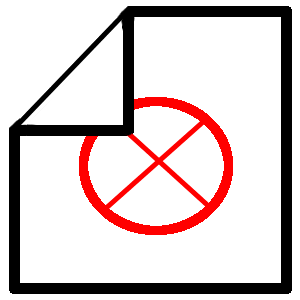
\includegraphics[width=0.2\textwidth]{dummy.png} % <- formatos PNG, JPG e PDF
	\fonte{ABNTEX, 2009\nocite{abnTeX2009}}
	\label{fig:dummy}
\end{figure}

\section{Tabelas}

Tamb\'em \'e apresentado o exemplo da Tabela~\ref{tab:correlacao}, que aparece automaticamente na lista de tabelas. Informa\c{c}\~oes sobre a constru\c{c}\~ao de tabelas no \LaTeX\ podem ser encontradas na literatura especializada~\cite{Lamport1986,Buerger1989,Kopka2003,Mittelbach2004}.

\begin{table}[!htb]
	\centering
	\caption[Exemplo de uma tabela]{Exemplo de uma tabela mostrando a correla\c{c}\~ao entre x e y.}
	\label{tab:correlacao}
	\begin{tabular}{c|c}
		\hline \SPACE
		\textbf{x} & \textbf{y} \\ \hline \SPACE
		1 & 2 \\ \hline \SPACE
		3 & 4 \\ \hline \SPACE
		5 & 6 \\ \hline \SPACE
		7 & 8 \\
		\hline 
	\end{tabular}
	\fonte{Pr\'oprio Autor.}
\end{table}

\section{Equa\c{c}\~oes}

A transformada de Laplace \'e dada na equa\c{c}\~ao~(\ref{eq:laplace}), enquanto a equa\c{c}\~ao apresenta a formula\c{c}\~ao da transformada discreta de Fourier bidimensional\footnote{Deve-se reparar na formata\c{c}\~ao esteticamente perfeita destas equa\c{c}\~oes!}.
\begin{equation}
X(s) = \int\limits_{t = -\infty}^{\infty} x(t) \, \text{e}^{-st} \, dt
\label{eq:laplace}
\end{equation}


\section{Siglas e s\'imbolos}

O pacote abn\TeX\ permite ainda a defini\c{c}\~ao de siglas e s\'imbolos com indexa\c{c}\~ao autom\'atica atrav\'es dos comandos {\ttfamily \textbackslash sigla\{\}\{\}} e {\ttfamily \textbackslash simbolo\{\}\{\}}. Por exemplo, o significado das siglas\sigla{CCECOMP}{Colegiado do Curso de Engenharia de Computa\c{c}\~ao},\sigla{DAEComp}{Diretório Acad\^emico de Engenharia de Computa\c{c}\~ao} e\sigla{UEFS}{Universidade Estadual de Feira de Santana} aparecem automaticamente na lista de siglas, bem como o significado dos s\'imbolos\simbolo{$\lambda$}{comprimento de onda},\simbolo{$v$}{velocidade} e\simbolo{$f$}{frequ\^encia} aparecem automaticamente na lista de s\'imbolos. Mais detalhes sobre o uso destes e outros comandos do abn\TeX\ s\~ao encontrados na sua documenta\c{c}\~ao espec\'ifica~\cite{abnTeX2009}.
